\section{Target group analysis}\label{sec:target-group-analysis}

Chess as a game has a broad appeal, as it is played by many people, young and old.
As previously stated, chess has risen in popularity recently, so it is sufficed to say that the user group is a lot
larger than it was a few years ago.
Therefore, it is necessary to analyze the target group to narrow down the scope of the problem.

A good way to do just that is by splitting the target group into different categories.
It is possible to split the people that play chess by age, skill level, and how frequently they play.
As the project is about the learning process of chess, the most relevant choice is to divide the target group based on
skill level.
To measure their skill level, the team uses the ELO rating system, which is a method for calculating the relative skill
levels of players in two-player games such as chess, using data from~\url{Chess.com}.

% textidote: ignore begin
\begin{figure}[H]
    \centering
    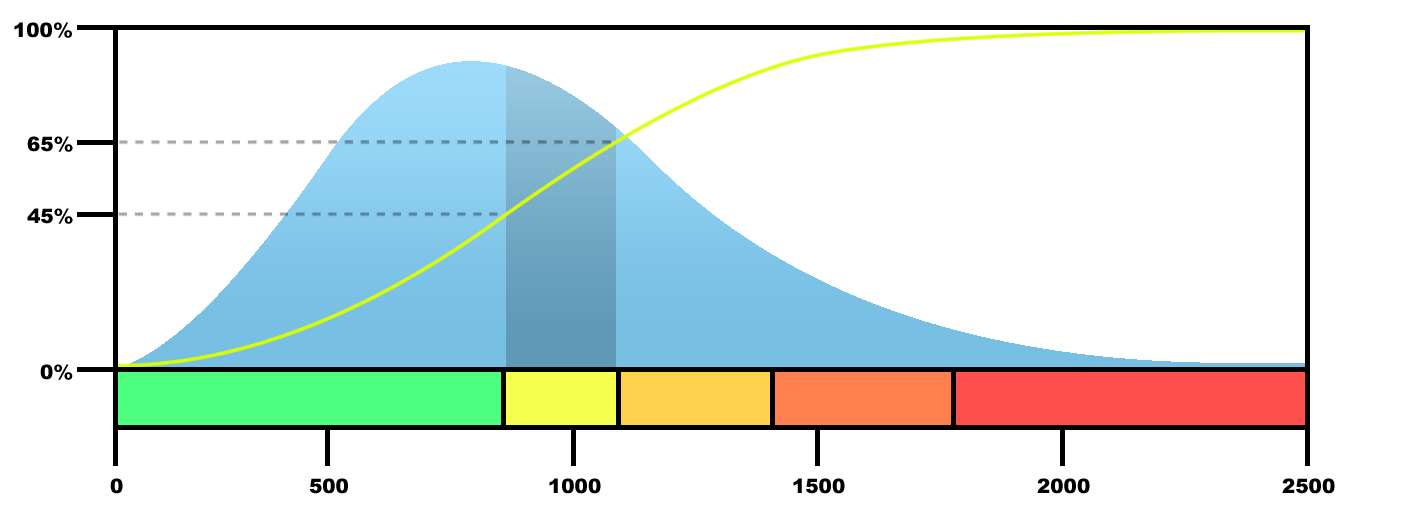
\includegraphics[width=1\textwidth]{chess-graph}
    \caption{Rating distribution graph based off of Chess.com's rating system~\cite{chess-ratings}.}\label{fig:graph}
\end{figure}
% textidote: ignore end

Figure~\ref{fig:graph} shows a graph made to illustrate different skill levels amongst the user base
of~\url{Chess.com}.
The blue wave represents the number of users with a certain rating.
The team doesn't have direct numbers as the graph is very limited in terms of data.
The color bars on the bottom represent different skill groups~\cite{chess-ratings}.

The first group, which is marked in green and is the biggest one, is novices.
They are not expected to know much about chess or its rules.
This is why they are not fit to be the target group, as the goal is not to teach the rules of chess, but rather to help
people improve their skills.
The second group, which is marked in yellow, is beginners.
This is the main target group, as they are the ones that are expected to benefit the most from the project.
That's because the graph peaks at the end of the novices group, which means that transitioning from novice to beginner
seems to be the hardest challenge for new players.
The team has therefore decided to focus on this group; to help them overcome this obstacle.
By focusing on this group, the team hopes to flatten the curve and make the transition from beginner to intermediate
easier.
The third and fourth groups, which are marked in light and dark orange, are intermediate one and two players.
While they are not the main target group, they may still have a subset of the problems that the beginners have.
Therefore, they can still benefit from the project.
The last group, which is marked in red, is expert players.
Unlike intermediate players, they are less likely to have the issues that the beginners have.

The yellow line shows the cumulative percentage of the data as the graph approaches the right.
It signals that the target group encapsulates all users between the 45th and the 65th percentile, which corresponds to
at least 20\% of blitz users on~\url{Chess.com}~\cite{chess-ratings}.
